\section{Sort}
\label{sort}

Sorting is among the most commonly used operations in database systems underlying operators like merge join, order by and occasionally group-by.  The process of sorting is quite write-intensive since the commonly used in-memory sorting algorithms, like \textit{quicksort}, involve a lot of data movement. In the single pivot quicksort algorithm with $n$ elements, the average number of swaps is of the order of $0.3nln(n)$ \cite{swaps}. There are other algorithms such as \textit{selection sort} which involve much lesser data movement but they incur quadratic time complexity in the number of elements to be sorted; thereby falling out of favour for large datasets.

We propose an in-memory sorting algorithm that leverages the idea of \textit{single-pivot} quicksort for partitioning the input data into separate ranges. The basic idea is to use multiple pivots to divide the data into smaller ranges for reducing the writes while retaining the time complexity of the single-pivot algorithm. We term the algorithm as \textit{multi-pivot sort}. In the following subsections, we begin by presenting the conventional single pivot quicksort case and subsequently cover the multi-pivot algorithm and its variations.

\subsection{Conventional quicksort}
The conventional quicksort algorithm begins by choosing one of the input elements as a pivot. Each pass divides the input array into two partitions, one partition containing elements lesser than the pivot, and the other containing those that are greater. This is achieved by means of in-place swapping of elements in the array. This partitioning is done recursively for the obtained partitions to give the final sorted array.

If the initial array was much larger than DRAM size, there would be DRAM evictions during the swapping process of partitioning. These evictions might lead to PCM writes if the evicted DRAM lines are \textit{dirty} (which is likely since elements are being swapped). If the resulting partitions sizes continue to be larger than DRAM, partitioning them in turn will again cause DRAM evictions and consequent writes. Clearly, this trend of writes will continue in the recursion tree until the partition sizes of the obtained partitions are small enough to fit within DRAM. Thereafter, there would be no evictions during swapping and the entire subsequent sorting process will finish within DRAM.

\begin{figure}
\centering
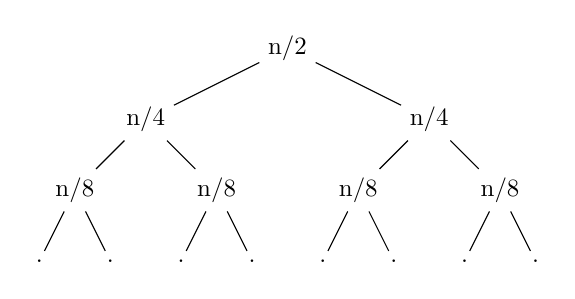
\begin{tikzpicture}[scale=.9, transform shape]

\tikzstyle{every node} = [rectangle, fill=gray!0]

\node (s) at (1,0) {.};
\node (t) at (2,0) {.};
\node (u) at (3,0) {.};
\node (v) at (4,0) {.};
\node (w) at (5,0) {.};
\node (x) at (6,0) {.};
\node (y) at (7,0) {.};
\node (z) at (8,0) {.};

\node (a) at (1.5,1) {n/8};
\node (b) at (3.5,1) {n/8};
\node (c) at (5.5,1) {n/8};
\node (d) at (7.5,1) {n/8};

\node (e) at (2.5,2) {n/4};
\node (f) at (6.5,2) {n/4};

\node (g) at (4.5,3) {n/2};

\draw[-] (s) -- (a);
\draw[-] (t) -- (a);
\draw[-] (u) -- (b);
\draw[-] (v) -- (b);
\draw[-] (w) -- (c);
\draw[-] (x) -- (c);
\draw[-] (y) -- (d);
\draw[-] (z) -- (d);

\draw[-] (a) -- (e);
\draw[-] (b) -- (e);
\draw[-] (c) -- (f);
\draw[-] (d) -- (f);

\draw[-] (e) -- (g);
\draw[-] (f) -- (g);
\end{tikzpicture} 
\caption{Recursion tree for quicksort writes}
\label{fig:rec_tree}
\end{figure}

\textbf{PCM write analysis}: 
Given an array with randomly permuted $N_R$ elements, let us assume the chosen pivot in each phase of recursion is the median of the partition elements. Since the elements are arranged randomly, the probability that the element is in the right partition is $1/2$. In other words, $n/2$ elements are expected to be incorrectly placed.

If Hoare partitioning \cite{cormen} is used, wherein each misplaced element is swapped with another misplaced element. moving these elements to their right partitions will incur $n/2$ writes. In the next level of the recursion tree, there will be $n/4$ writes for both the partitions, again totalling to $n/2$. Thus, $n/2$ writes for swaps will continue until the size of the partition reaches to less than $D$, i.e when the level $l = \lceil log_2 (\frac{N_R L_R}{D}) \rceil$. After this, there would simply be $N_R L_R$ writes for writing each each sorted partition. This recursion tree is shown in Figure \ref{fig:rec_tree}. Totalling this across all levels, we get:
\begin{equation}
\label{eq:sort_conv}
\begin{split}
W_{sort\_conv} = 0.5N_RL_R \lceil log_2(\frac{N_R L_R}{D}) \rceil + N_R L_R\\
  = N_RL_R (0.5 \lceil log_2(\frac{N_R L_R}{D}) \rceil + 1) \\
\end{split}
\end{equation}



\begin{comment}
In the quicksort algorithm on randomly permuted $N_R$ tuples, the average number of swaps is $0.33N_Rln(N_R)$ \cite{swaps}. If each pair of swapped tuples gets evicted from DRAM to PCM after each intermediate swap, there will be two tuple writes (of $L_R$ bytes each) in PCM per pair of swapped tuples. Hence, the total number of writes is given by:  
\end{comment}
\subsection{Multi-pivot quicksort}
\label{subsec:sort_mpivot}
It is clear from the discussion on conventional sorting that, in terms of writes, the faster we converge to partition sizes within DRAM size, the better. A limitation of the conventional quicksort algorithm is that partitioning using a single pivot leads to just two partitions. Thus, with each recursive step in quicksort, the partition size is at best halved (assuming selecting the median as the pivot each time). The intuition behind the multi-pivot quicksort algorithm is to get past this limitation of single-pivot quicksort by using multiple pivots instead, so that the individual partitions quickly converge to a size lesser than the DRAM size.

However, in the multi-pivot case, we do not have any prior information about the endpoints of the partitions to facilitate direct movement of elements to their respective partitions during partitioning, as is done in single pivot quicksort. We address this limitation by adding a separate \textit{read phase} that makes an initial read pass over the input elements counting the number of elements between each consecutive pair of pivots. Note that these counters, by virtue of being continuously updated during the read pass, are likely to be updated within DRAM itself, not incurring PCM writes. After this pass, we are equipped with the endpoint information necessary for the subsequent phases of the algorithm.

We now present an exposition of the various phases of the multi-pivot quicksort algorithm:

\subsubsection{Read phase} 



In the read phase, we divide the input tuples into $p$ partitions of approximately D size each s.t. $p = \lceil \frac{N_R L_R}{D} \rceil$ by choosing $p-1$ random tuples as pivots. These pivots are then copied to a separate location and sorted. Subsequently, we scan through the tuples array counting the number of elements between each consecutive pair of pivots. This is accomplished by doing a binary search within the sorted list of pivots for each tuple in the array. Algorithm \ref{alg:read_phase} represents the pseudo-code for the read phase.

\begin{algorithm}
%{\fontsize{8pt}{10pt}\selectfont
\caption{Read Phase}
\label{alg:read_phase}
\textbf{c} is a design parameter\\
\begin{algorithmic}[1]
\State p = $\lceil c\times \frac{N_R L_R}{D} \rceil$;
\State randIndex[] = generate $p-1$ random indexes;
\State pivot[] = a[randIndex];
\State size[] = {0..0};   
\Comment{size of sub-arrays}
\For {i=$1$ to $N_R$}
\State partition = getPartition(array[i]) 
\State size[partition]++ 
\EndFor
\Comment {Time complexity=$N_R\times log_2p$ }
\State Calculate the boundary index of sub-arrays using their size.
\State return sub-arrays boundary indexes;
\end{algorithmic}
%}
\end{algorithm}


\subsubsection{Swap phase} 
The swap phase uses the information gathered in the read phase to group tuples of the same partition together. The algorithm for swap phase is shown in Fig \ref{alg:swap_phase}. The algorithm operates in a manner similar to cycle-sort, writing each entry directly to its correct partition in-place. 

The algorithm first picks up a wrongly placed entry $e_1$ in a partition $P_1$ and determines it's correct partition $P_2$ by comparing it with the pivots. It then finds another wrongly placed entry $e_2$ belonging to partition $P_2$ and writes $e_1$ in its place. Now the correct partition $P_3$ of $e_2$ is determined and a misplaced element $e_3$ is identified from $P_3$ as a victim for replacement. The algorithm proceeds in the same manner till the cycle completes with the last incorrectly placed entry belonging to partition $P_1$. The algorithm keeps initiating such cycle of replacements till all the elements are placed in their correct partitions. This is reminiscent of the the cycle-sort algorithm \cite{cycle_sort}.

The pseudo-code for swap phase is shown in Algorithm \ref{alg:swap_phase}. The writes during this phase cannot exceed $N_R L_R$ since in the worst case, \emph{each} tuple would have to be moved to its correct partition.

\begin{algorithm}[h!]
%{\fontsize{8pt}{10pt}\selectfont
\caption{Swap Phase}
\label{alg:swap_phase}
partitionStart[] and partitionEnd[] are obtained from Read Phase
\begin{algorithmic}[1]
\For {i=1 to $N_R$}
	\State partitionCorrect = getPartition(array[i])
     \If {i between partitionStart[partitionCorrect] and partitionEnd[partitionCorrect]}                
     \State partitionStart[partitionCorrect]++
	\State continue;
     \Else
			\State presentVictim = a[partitionStart[partitionCorrect]]             
            \State a[partitionStart[partitionCorrect]] = a[i]
            \State partitionStart[partitionCorrect]++
            \State flag = 1;
            \While {flag} 
                \State partitionStart = partitionStart[partitionCorrect];
                \State partitionEnd = partitionStart[partitionCorrect + 1];
                \State partitionLast = partitionCorrect;
                \For {k=partitionStart to partitionEnd} 
                \State partitionCorrect = getPartition(array[i]);
                    \If {k between partitionStart[partitionCorrect] and  partitionStart[partitionCorrect + 1]}
                        \State continue;
                        
                    \ElsIf {k == firstVictimLoc} 
                        \State flag = 0;
                    \EndIf
                    \State swapTuples(presentVictim, array + (arrayElemSize * k));
                    \State currPartitionPtr[partitionLast] = k;
                    \State break;
             
				\EndFor
			\EndWhile
	\EndIf
\EndFor
\Comment {Time complexity=$N_R\times log_2p$ }
\end{algorithmic}
%}
\end{algorithm}


\subsubsection{Sort phase}
Finally, each of the partitions are sorted separately using conventional quicksort to get the final PCM sorted array. If all the partitions are within the DRAM size, the sort phase for each partition can potentially finish within the DRAM without any intermediate evictions to PCM. 

\begin{algorithm}
%{\fontsize{8pt}{10pt}\selectfont
\caption{Sort Phase}
\label{alg:sort_phase}
\begin{algorithmic}[1]
\For {i=$1$ to $p$}
\If {size[p] < D}
\State quicksort(partition $p$)
\Else 
\State multi-pivot quicksort(partition $p$)
\EndIf 
\EndFor
\end{algorithmic}
%}
\end{algorithm}

A point to note here is that since we are choosing the pivot values randomly, it is likely that some partitions turn out to be larger than DRAM. We account for this possibility by creating extra partitions. This is done by selecting a constant c (a value of 2 was found to work well experimentally) s.t. now $p = \lceil c \times \frac{N_R L_R}{D} \rceil$. Post the read phase, we identify the adjoining underflow partitions and coalesce them if their total size is within the DRAM size, after leaving some space for bookkeeping information. If some large partitions still remain, we recursively apply the multi-pivot quicksort algorithm to sort them. Smaller partitions, on the other hand, are sorted using the conventional quicksort, since the sorting process is expected to finish within DRAM and hence not cause any intermediate evictions. 

Figure \ref{fig:mpsort} represents all the steps in the sorting of a given input array for multi-pivot quicksort. In the read phase, 30 and 15 are chosen as pivots. These pivots divide the input elements into 3 different ranges: $< 15$, $\geq 15$ and $< 30$, $\geq 30$. The count of elements in each of these ranges is then determined by making a pass over the elements. In the swap phase, the elements are moved to within the boundaries of their respective partitions. The sort phase finally sorts each of these partitions separately.


%\newcolumntype{b}{>{\columncolor{white}}c}
\begin{figure}[h]
	\centering
	\subfloat[Read Phase]{	
  	%\includegraphics[width=8cm]{sort_step_1.png}
  	
  	\begin{tabular}{|c|c|c|y|c|y|c|c|c|}
        \hline
        24&3&33&30&21&15&7&32&11\\\hline
    \end{tabular}
    }
	\hspace{0mm}
	\subfloat[Swap Phase]{
  	\begin{tabular}{|x|x|x|y|y|y|z|z|z|}
        \hline
        11&3&7&24&21&15&33&32&30\\\hline
    \end{tabular}
    }
    \hspace{0mm}
	\subfloat[Sort Phase]{
  	\begin{tabular}{|x|x|x|y|y|y|z|z|z|}
        \hline
        3&7&11&15&21&24&30&32&33\\\hline
    \end{tabular}
    }
	\caption{Multi-Pivot Sort}
	\label{fig:mpsort}
	
\end{figure}
\textbf{PCM write analysis}: Though the partition boundary counters are continuously updated during the Read phase, they are expected to incur very few PCM writes. This is because since all those updates are in quick succession, the counters are unlikely to be evicted from DRAM  \emph{during} the update process. Similarly, negligible writes would be incurred during extracting and sorting the pivots. During the Swap phase, there will be $N_R L_R$ writes since each tuple is written only once while placing it within its partition boundaries. If each partition is within the DRAM size, the Sort phase (for each partition) will finish within DRAM and there will be another $N_R L_R$ upon eventual eviction of sorted partitions to PCM.  Thus, the total writes in this algorithm is be given by 
\begin{equation}\label{eq:mpivot}
  W_{mpivot} = 2N_RL_R
\end{equation}

\subsection{Multi-pivot sort without explicit partitioining}
The multi-pivot algorithm discussed in the previous section incurred $N_R L_R$ writes during the swap phase due to materialization of partitions in-place. If the available PCM size is sufficient to accommodate another copy of the array to be sorted, we can avoid partitioning writes by trading the swap phase for multiple \textit{sort} passes, each pass carrying out the sorting one of the partitions in the array using the additional space available. This space eventually feeds the sorted tuples as input to the parent operator in the query plan tree. 

In each pass, we go over the entire array, copying the elements belonging to one partition to the space and subsequently sort them there, before moving to the next partition. The process of copying would seem to incur writes of itself and would thus apparently be self-defeating. However, in this case, we leverage the DRAM replacement policy by choosing an appropriate partition size which would prevent dirty (written) words from getting evicted. For N-Chance replacement policy, such a partition size would be $\frac{(N-1)}{K}\times D$. This would ensure that the extracted partition elements do not get evicted before sorting finishes for the partition. In this manner, each partition is processed sequentially by making multiple passes over the entire input array.

\textbf{PCM write analysis}: In this scheme, since there are no extraction writes, the writes incurred are just due to the eviction of the sorted partitions from DRAM. Thus the total writes are given by 
\begin{equation}\label{eq:mpivot_wep}
  W_{mpivot_wep} = N_RL_R
\end{equation}